\documentclass[border=4pt,varwidth=17cm]{standalone}
\usepackage{amsmath,amssymb,mathrsfs,mathtools}
\usepackage{tikz}
\usetikzlibrary{positioning,fit,backgrounds,arrows.meta}
\def\RR{{\mathbb R}}\def\eps{\varepsilon}\def\then{\Rightarrow}
\def\J{\mathcal{J}_L}\def\A{\mathcal{A}_{f,g}}\def\Sol{\mathcal{S}_{f,g}}
\def\limsup{\mathop{\overline{\lim}}}\def\liminf{\mathop{\underline{\lim}}}
\def\Of{{\sf (O$_f$)}}\def\Og{{\sf (O$_g$)}}
\def\Rv{{\sf (R$_{\rm v}$)}}\def\Rh{{\sf (R$_{\rm h}$)}}
\begin{document}


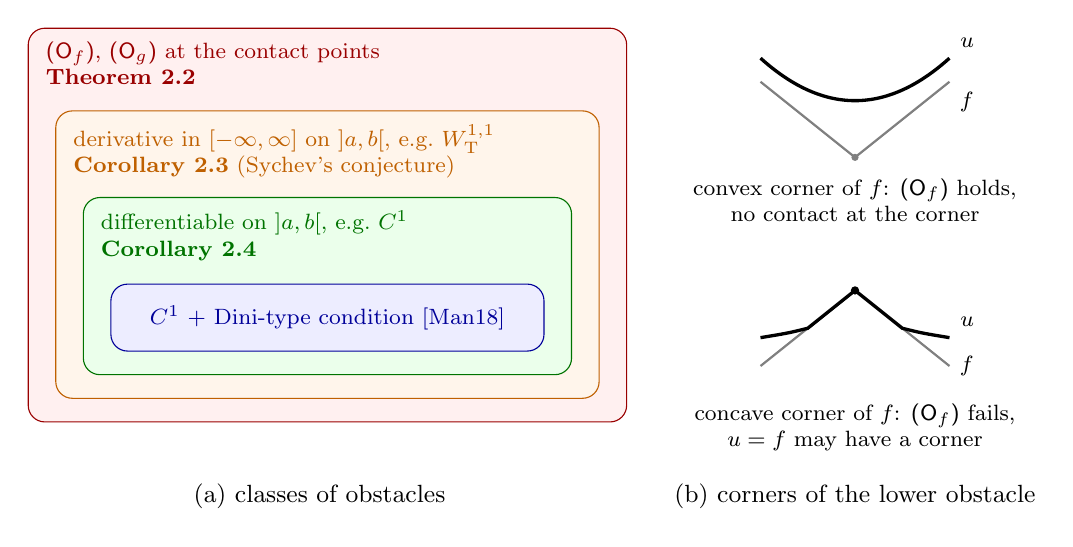
\begin{tikzpicture}[font=\footnotesize]
% ---------- (a) classes of obstacles
\begin{scope}
  \draw[rounded corners=6pt, draw=red!60!black, fill=red!6] (0,0) rectangle (7.6,5.0);
  \node[anchor=north west, align=left, text=red!60!black] at (0.1,4.95) {\Of, \Og\ at the contact points\\ \textbf{Theorem 2.2}};
  \draw[rounded corners=6pt, draw=orange!75!black, fill=orange!8] (0.35,0.3) rectangle (7.25,3.95);
  \node[anchor=north west, align=left, text=orange!75!black] at (0.45,3.9) {derivative in $[-\infty,\infty]$ on $]a,b[$, e.g.\ $W^{1,1}_{\rm T}$\\ \textbf{Corollary 2.3} (Sychev's conjecture)};
  \draw[rounded corners=6pt, draw=green!45!black, fill=green!8] (0.7,0.6) rectangle (6.9,2.85);
  \node[anchor=north west, align=left, text=green!45!black] at (0.8,2.8) {differentiable on $]a,b[$, e.g.\ $C^1$\\ \textbf{Corollary 2.4}};
  \draw[rounded corners=6pt, draw=blue!60!black, fill=blue!7] (1.05,0.9) rectangle (6.55,1.75);
  \node[align=center, text=blue!60!black] at (3.8,1.325) {$C^1$ + Dini-type condition [Man18]};
  \node[font=\small] at (3.7,-0.95) {(a) classes of obstacles};
\end{scope}
% ---------- (b) convex corner of f
\begin{scope}[shift={(10.5,3.6)}, x=1.2cm, y=1.2cm]
  \draw[thick, gray] (-1,0.6) -- (0,-0.2) -- (1,0.6) node[below right, black] {$f$};
  \draw[very thick, domain=-1:1, samples=40, smooth] plot (\x, {0.4+0.45*\x*\x}) node[above right] {$u$};
  \fill[gray] (0,-0.2) circle (1.3pt);
  \node[align=center] at (0,-0.65) {convex corner of $f$: \Of\ holds,\\ no contact at the corner};
\end{scope}
% ---------- (c) concave corner of f
\begin{scope}[shift={(10.5,0.95)}, x=1.2cm, y=1.2cm]
  \draw[thick, gray] (-1,-0.2) -- (0,0.6) -- (1,-0.2) node[right, black] {$f$};
  \draw[very thick] (-1,0.1) .. controls (-0.7,0.15) .. (-0.5,0.2) -- (0,0.6) -- (0.5,0.2) .. controls (0.7,0.15) .. (1,0.1) node[above right] {$u$};
  \fill (0,0.6) circle (1.5pt);
  \node[align=center] at (0,-0.85) {concave corner of $f$: \Of\ fails,\\ $u=f$ may have a corner};
\end{scope}
\node[font=\small] at (10.5,-0.95) {(b) corners of the lower obstacle};
\end{tikzpicture}


\end{document}
